\documentclass[11pt]{handout}
\usepackage{moreverb}
\usepackage{tabularx}
\usepackage{epsf}
\usepackage{epsfig}
\usepackage{fancyheadings}
\usepackage{fancybox}

\renewcommand{\coursetitle}{ECE 320}
\renewcommand{\handouttitle}{Speech Coding}
\renewcommand{\handoutauthor}{Swaroop Appadwedula}
\renewcommand{\semestertitle}{Spring 2000}

\newcommand{\bea}{\begin{eqnarray}}
\newcommand{\eea}{\end{eqnarray}}

\setlength{\parindent}{5mm}
\begin{document}

\setlength{\baselineskip}{0.5cm}
\setlength{\parskip}{0.5cm}

\makeboxtitle
\vspace{0.3cm}

\section{Introduction}
In this project lab, you will implement a linear predictive coder 
for speech.  After recording speech signals, you will write 
\matlab code to implement the Levinson-Durbin algorithm, as well as 
assembly code to compute autocorrelation coefficients for overlapped 
blocks.

%
% Module: lpc_theory_tutorial
%
% Author: Swaroop Appadwedula, Jan. 21, 2001
%
%

\subsection{Correlation Coefficients}
To measure the degree of similarity between two signals, we can
compute their correlation.  The cross-correlation between two
discrete-time signals $x(n)$ and $y(n)$ is defined as
\begin{equation}
      r_{xy}(l) = \sum_{n=-\infty}^{\infty}x(n)y(n-l)
\end{equation}
where $n$ is the sample index, and $l$ is the lag or time
shift between the two signals \cite{Proakis} (p.120).  Since 
speech signals are not stationary, we are typically interested 
in the similarities between signals only over a short time 
duration ($<30ms$).  In this case, the cross-correlation 
is computed only over a window of time samples and for only 
a few time delays $l = 0,1,\dots,P$.  Consider the 
autocorrelation sequence $r_{ss}(l)$, which describes the 
redundancy in the signal $s(n)$.
\begin{equation}
      r_{ss}(l) = \frac{1}{N}\sum_{n=0}^{N-1}s(n)s(n-l)
\label{equ:autocorrelation}
\end{equation}
where $s(n)$, $n=-P,-P+1,\ldots,N-1$ are the known 
samples (see Figure \ref{fig:correlation}) and the $\frac{1}{N}$ is 
a normalizing factor.

\begin{figure}[htb]
   \begin{center}
      
\epsfig{file=correlation.eps,width=6cm}
      \vspace*{0.5cm}
      \caption{Computing the autocorrelation coefficients}
      \label{fig:correlation}
   \end{center}
\end{figure}

Another related method of measuring the redundancy in a signal is to 
compute its autocovariance
\begin{equation}
        r_{ss}(l) = \frac{1}{N-l}\sum_{n=l}^{N-1}s(n)s(n-l)
\label{equ:autocovariance}
\end{equation}
where the summation is over $N-l$ products (the samples 
$s(-P),\ldots,s(-1)$ are ignored).
%It is known that for speech 
%signals, using the autocovariance coefficients has better stability for 
%linear prediction.

\subsection{Linear Prediction Model}
Linear prediction is a good model for recognition of 
speech signals.  In linear prediction, the human vocal tract 
is modeled as an infinite impulse respone (IIR) system that produces 
the speech signal.  For vowel sounds and other voiced regions of speech, 
which have a resonant structure and high degree of similiarity over 
particular time shifts, this modeling produces an efficient 
representation of the sound.  Figure \ref{fig:lpc model} shows how the 
resonant structure of a vowel could be captured by an IIR system.

\begin{figure}[htb]
  \begin{center}
      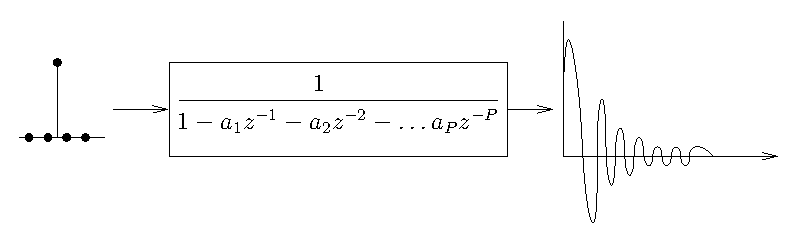
\epsfig{file=lpc_model.eps,width=12cm}
      \vspace*{1.5cm}
      \caption{Linear Prediction (IIR) Model of Speech}
      \label{fig:lpc model}
  \end{center}
\end{figure}


The linear prediction problem can be stated as finding the 
coefficients $a_k$ which result in the best prediction (which minimizes 
mean-squared prediction error) of the speech sample $s(n)$ in terms of 
the past samples $s(n-k)$, $k=1,\ldots,P$.  The predicted sample 
$\hat{s}(n)$ is then given by \cite{Rabiner}
\begin{equation}
        \hat{s}(n) = \sum_{k=1}^{P} a_k s(n-k)
\label{equ:prediction}
\end{equation}
where $P$ is the number of past samples of $s(n)$ which we wish to
examine.  Now, we derive the frequency response 
of the system in terms of the prediction coefficients 
$a_{k}$ as follows.  In (\ref{equ:prediction}), when the predicted sample 
equals the actual signal (i.e $\hat{s}(n) = s(n)$), we have
\begin{eqnarray}
        s(n) & = & \sum_{k=1}^{P} a_k s(n-k)    \nonumber \\
        S(z) & = & \sum_{k=1}^{P} a_k S(z)z^{-k}    \nonumber \\
        S(z) & = & \frac{1}{1 - \sum_{k=1}^{P}a_{k}z^{-k}}
\label{equ:IIR}
\end{eqnarray}
The optimal solution to this problem is \cite{Rabiner}
\begin{eqnarray}
        {\bf a} & = & \left[a_1 \,\, a_2 \,\, 
                        \ldots \,\, a_P \right] \nonumber \\
        {\bf r} & = & \left[r_{ss}(1)\,\, r_{ss}(2) \,\, 
                        \ldots \,\, r_{ss}(P) \right]^{T} \nonumber \\
        {\bf R} & = & \left(\begin{array}{c c c c c c}
        r_{ss}(0) & r_{ss}(1) & \ldots & r_{ss}(P-1) \nonumber \\ 
        r_{ss}(1) & r_{ss}(0) & \ldots & r_{ss}(P-2)  \nonumber \\
        & & \vdots \nonumber \\
        r_{ss}(P-1) & r_{ss}(P-2) & \ldots & r_{ss}(0) \nonumber \\
        \end{array}\right) \nonumber \\
        {\bf a} & = & {\bf R}^{-1}{\bf r}
\end{eqnarray}
Due to the Toeplitz property (symmetric with 
equal diagonal elements) of the ${\bf R}$ matrix, an efficient 
algorithm is available for computing ${\bf a}$ without finding 
${\bf R}^{-1}$.  Levinson's algorithm is an iterative method of 
computing the predictor coefficients ${\bf a}$ \cite{Rabiner} (p.115).

\vspace*{0.5cm}
\begin{tabular}{l l l}
Initial Step  &: $E_{0} = r_{ss}(0), i=1$\\
for i := 1 to P \{ \\
       &Step 1&: $k_{i} = \frac{1}{E_{i-1}}\left( r_{ss}(i) - 
                \sum_{j=1}^{i-1}\alpha_{j,i-1}r_{ss}(i-j) \right)$ \\ 
       &Step 2&: $\alpha_{j,i} = \alpha_{j,i-1} - k_{i}
                                  \alpha_{i-j,i-1}\,\,\,  
                                                j =1,\ldots,i-1$\\
       &     &\,\, $\alpha_{i,i} = k_{i}$\\
       &Step 3&: $E_{i} = (1-k_{i}^2)E_{i-1}$\\ 
\}
\end{tabular}
\vspace*{0.5cm}

\subsection{LPC-based Synthesis (Optional)}
Use the prediction coefficients to synthesize the original sound by 
applying $\delta(n)$, the unit impulse, to the IIR system with 
lattice coefficients $k_{i}$, $i=1,\ldots,P$ as shown in 
Figure \ref{fig:lattice}.  Apply 
$\delta(n)$ to consecutive IIR systems (which represent consecutive 
speech segments) to get a longer segment of synthesized speech.  

In this application, lattice filters are used rather than 
direct-form filters since they provide a good representation of 
the reflections in the vocal tract.  Lattice filters have 
coefficients with magnitude less than $1$ and are available 
directly as a result of the Levinson-Durbin algorithm.  If a 
direct-form implementation is desired, the $\alpha$ coefficients 
would need to be factored into second-order stages with 
very small gains to yield a more stable implementation.

\begin{figure}[ht]
   \begin{center}
      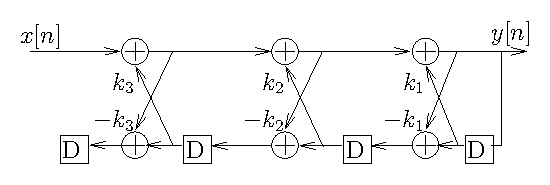
\epsfig{file=lattice.eps,width=9cm}
      \vspace*{0.5cm}
      \caption{IIR lattice filter implementation.}
      \label{fig:lattice}
   \end{center}
\end{figure}

When each segment of speech is synthesized in this manner, two problems 
occur.  First, the resulting synthesis is monotone and contains no 
changes in pitch since the $\delta(n)$ are input with the fixed 
periodicity equal to the segment length.  Second, the states of the 
lattice filter (values in the delay boxes) are cleared at the 
beginning of each segment, causing discontinuity in the output.

To recover the pitch, we look at the autocorrelation coefficients of 
each segment.  A large peak in the autocorrelation coefficient at 
lag $l\neq0$ would correspond to a periodicity $l$ of the speech 
in that segment.  If the speech segment does not have a large peak 
in the autocorrelation coefficients, then the segment is an 
unvoiced signal which has no periodicity.  Unvoiced segments such as 
consonants are best reconstructed by inputting noise into the IIR 
model.  For voiced segments such as vowels, an impulse train 
with delay between impulses varied according to the pitch period 
in each segment provides a good approximation to the originial pitch 
variation.

To reduce the discontinuity between segments, do not clear the 
states of the IIR model from one segment to the next.  Instead, load 
the new set of reflection coefficients, $k_i$, and continue with the 
lattice filter computation.

\begin{thebibliography}{2}

\bibitem{Proakis}
J.~G. Proakis and D.~G.Manolakis, {\em Digital Signal Processing: 
Principles, Algorithms, and Applications}.
\newblock Upper Saddle River, NJ: Prentice-Hall, 1996.

\bibitem{Rabiner}
L.Rabiner and B.-H. Juang, {\em Fundamentals of Speech Recognition}.
\newblock Englewood Cliffs, NJ: Prentice-Hall, 1993.

\end{thebibliography}



\section{Matlab Exercises}

%AUTHOR: Swaroop Appadwedula
\paragraph{Exercise}
Take a simple signal (e.g. one period of a sinusoid at some frequency) 
and plot its autocorrelation sequence for appropriate values of $l$.  
You may wish to use the \verb+xcorr+ \matlab function to
compare with your own version of this function.  At what time
shift $l$ is $r_{ss}(l)$ maximized and why?  Is there any
symmetry in $r_{ss}(l)$?  What does $r_{ss}(l)$ look like for
periodic signals?

\paragraph{Exercise}
Write your own version of the Levinson-Durbin algorithm in \matlab.  
Note that \matlab uses indexing from $1$ rather than $0$.  A good idea 
would be to start the loop with $i=2$, and appropriately shift 
the variables $k, E, \alpha$, and $r_{ss}$ to start at $i=1$ and 
$j=1$. Be careful with indices such as $i-j$, since these could 
still be $0$.  

Apply your algorithm to a $20-30ms$ segment of a speech signal.  
Use the small powered microphone or professional microphone
available in the DSP lab to record \verb+.wav+ audio files on the
PC using the application Sound Recorder.  Typically, a
sampling rate of $8kHz$ is a good choice
for voice signals which have maximum
frequency below $4kHz$.  
You will use these audio files to test algorithms in  
\matlab.  The following functions will help you
read, write and play audio files in \matlab:
\verb+wavread,wavwrite,sound+.  You can also convert CD
tracks to a \verb+.wav+ file using the Mediaplayer application
on the PC.

The output of the algorithm is the prediction coefficients $a_k$ 
(usually about $P=10$ coefficients is sufficient), 
which represent the speech segment containing significantly 
more samples.  The LPC coefficients are a compressed representation 
of the ordinal speech segment.  Compare the 
coefficients generated by your function with those generated 
by the \verb+levinson+ or \verb+lpc+ functions available in the 
\matlab toolbox.  Next, plot the frequency response of the IIR model 
represented by the LPC coefficients where 
$a_{k} = \alpha_{k,P}, k=1,2\ldots,P$ (see (\ref{equ:IIR})).  
What is the fundamental frequency of the speech segment?  Is 
there any similarity in the prediction coefficients for 
different $20-30ms$ segments of the same vowel sound? 
How could the prediction coefficients be used for recognition?



\section{Implementation}

%AUTHOR: Swaroop Appadwedula
However, the sampling rate on the 6-channel 
DSP boards is fixed at $44.1kHz$, so decimation of $5$ may be used 
to achieve the sampling rate of $8.82kHz$.  

Using either the test vector thru code or the input-output thru code, 
compute the autocorrelation or 
autocovariance coefficients of $256$-sample blocks of input samples from 
the function generator for time shifts $l=0,1,\ldots,15$ (i.e. $P=15$) and 
display these on the oscilloscope with a trigger.  (You may zero out 
the other $240$ output samples to fill up the $256$ sample block).  
For computing the autocorrelation, 
you will have to use memory to record the last $15$ samples of the input 
due to the overlap between adjacent blocks.  
Compare the output on the oscilloscope with the results from \matlab.

The next step is to use a speech signal as the input to your system.  
Use the powered microphone as the input to the original
\verb+thru.asm+ code and adjust the gains in your system until 
the output has reasonable amplitude and does not saturate.  
Now, you will need to write code to determine 
the start of a speech signal, record a few seconds of speech and 
compute the autocorrelation or autocovariance 
coefficients.  
In order to make a fair comparison with your \matlab version (with
speech sampled at $8 kHz$) you will have to resample the input.
A decimation factor of $5$ on the DSP is suggested resulting in a 
a sampling rate of $8.82 kHz$ for your speech input.
The start of a speech signal can be determined by comparing 
the input to some noise threshold.  For recording large segments of 
speech, you may need to use external memory. Refer to the handout on 
external memory for more information.

Finally, incorporate your code which computes autocorrelation or 
autocovariance coefficients with the code which takes speech 
input and compare the results seen on the oscilloscope to those 
generated by \matlab.

\paragraph{Optional}
In order to implement the Levinson-Durbin algorithm, you will need to 
use integer division to do Step 1 of the algorithm.  
Refer to the 54x Applications Guide and the \verb+subc+ 
instruction for a routine that performs integer division.



\section{Additional Issues}
\begin{itemize}
\item{Spanish vowels are easier to recognize using LPC.}
\item{Compute error as ${\bf a}^{T}{\bf R}{\bf a}$, 
      where ${\bf R}$ is the autocovariance or autocorrelation matrix 
      of a test segment and ${\bf a}$ is the vector of prediction 
      coefficients of a template segment.}
\item{Use a pre-emphasis filter before LPC to emphasize frequencies of 
      interest in the recognition or synthesis.}
\item{The pitch period for males (80-150 Hz) is different than the 
      pitch period of females.}
\item{For voiced segments, $\frac{r_{ss}(T)}{r_{ss}(0)} \approx 0.25$, 
      where $T$ is the pitch period.}
\end{itemize}

\bibliographystyle{ieeetr}
\bibliography{../../ece320}

\end{document}

\bye
